

\section{Diskussion}
\label{sec:Diskussion}

Dieses Kapitel befasst sich mit der Diskussion der im \autoref{sec:auswertung} erhaltenen Ergebnisse.




Die Überprüfung der Resonatorstabilität ergab als maximale Resonatorlängen, die Werte

\begin{equation}
L_{max} = \text{204,0}\,\text{cm} \ \ \ \text{für}\  r_1, r_2 = 1400\,\text{mm}
\end{equation}
\begin{equation}
L_{max} = \text{139,5}\,\text{cm} \ \ \ \text{für}\  r_1 = \infty, r_2 = 1400\,\text{mm}
\end{equation}


Diese sind innerhalb der theoretisch möglichen Grenzen wie sie in \autoref{eq:Lmax1} und \autoref{eq:Lmax2} berechnet wurden. 
Der Wert von 204,0\,cm ist von der theoretischen Größe 76\,cm entfernt, da der Versuchsaufbau keine größere Resonatorlänge zuließ.
Der Messwert von 139,5\,cm liegt vergleichsweise sehr nahe am theoretischen Maximum. Abweichungen könnten durch Messungenauigkeiten zustande gekommen sein. So ist der Abstand zwischen den Befestigungspunkten der Spiegel sehr gut zu vermessen gewesen, der Abstand vom Befestigungspunkt zur Spiegeloberfläche jedoch nur sehr schwierig.\\
\\
Die transversalen Moden $\text{TEM}_{00}$ und $\text{TEM}_{10}$ ließen sich sehr gut beobachten.
\autoref{fig:TEM_00} zeigt, dass die Messwerte sehr gut dem Verlauf einer Gaußschen Kurve, wie sie von der Theorie vorhergesagt wird, folgen. Die sprunghaften Abweichungen einiger Messpunkte könnten die Empfindlichkeit der Photodiode als Ursache tragen, da selbst ein Auflegen der Hand auf die Fläche, auf der die Messapparturen stehen, zu einer merkbaren Änderung der gemessenen Stromstärke geführt hat.\\
Der Verlauf aus \autoref{fig:TEM_10} deckt sich gut genug mit dem theoretisch vorhergesagten. Deutlich zu erkennen ist jedoch, dass die Messwerte im negativen $\Delta x$-Bereich etwas zu niedrig, im positiven etwas zu hoch zu sein scheinen. Dies deutet auf einen systematischen Fehler hin. Etwa einen Winkel zwischen optischer Achse der Photodiode und der optischen Achse des Lasers, sodass Licht zu einer Seite der optischen Achse senkrechter in die Photodiode fällt als auf der anderen Seite. Eventuell könnte aber auch der Wolfram-Draht, der in den Resonator eingebracht wurde, nicht komplett mittig liegen und so eine Seite etwas mehr abschwächen als die andere. Zusammenfassend decken sich Theorie und Messung jedoch ausreichend genug, um die vorhergesagten Verläufe zu bestätigen.\\
\\
Für vollständig in einer Richtung polarisiertes Licht beträgt der Anteil der Amplitude, der parallel zur Durchlassrichtung des Polarisationsfilters liegt, gerade $\cos (\phi)$ der maximalen Amplitude. Der Winkel $\phi$ ist derjenige zwischen Polarisationsrichtung des Strahls und Durchlassrichtung des Filters. Da die Intensität proportional zum Quadrat der Amplitude ist, folgt damit der Verlauf der Lichtintensität einer $(\cos)^{2}(\phi)$ Kurve.\\
In \autoref{fig:Polarisation} ist zu sehen, dass der gemessene Verlauf der vorhergesagten Kurve sehr gut entspricht.
Damit konnte gezeigt werden, dass die vermessene Laserstrahlung vollständig Polarisiert ist.
 Der Winkel zwischen Polarisationsrichtung der Laserstrahlung und der Richtung, die auf dem Filter als 0\,° angezeigt wird, entspricht dem errechneten Parameter:

\begin{equation}
\phi_0 = (\text{86,82} \pm \text{0,15})\,\text{°}
\end{equation}


Die Anzahl der lontigudinalen Moden, die sich als stehende Wellen im Resonator entwickeln, ergibt sich aus der Resonatorlänge, aber auch der Verbreitung des Neon-Überganges durch den relativistischen Doppler-Effekt. Da die Anzahl der möglichen Moden mit der Resonatorlänge zunimmt, sollten auch mehr Schwebungsfrequenzen mit dem Spektrumanalysator messbar sein. An der \autoref{tab:Multimoden} ist erkennbar, dass für die drei größten Längen nur höhere Harmonische jeweils messbar waren. Dies führt auch zu den, im \autoref{sec:Multimodenbetrieb} erwähnten, Abweichungen dieser Messwerte, weshalb sie in der Auswertung schlussendlich weggelassen wurden. Auch die Messreihe zur kleinsten Resonatorlänge weicht stark ab und wurde am Ende ausgelassen. Weshalb dies der Fall ist, ist nicht absehbar.\\
Der berechnete Abstand zwischen zwei longitudinalen Moden ist nur von der Resonatorlänge abhängig. Die zum optimieren verwendete Funktion ließ sich sehr gut an die Messwerte anpassen. Der bestimmte Parameter
\begin{equation}
c_0 = (\text{299400884,188} \pm \text{9,146})\, \frac{\text{m}}{\text{s}}
\end{equation}
soll laut Theorie der Lichtgeschwindigkeit entsprechen. Die Abweichung zwischen dem Parameter $c_0$ und der Naturkonstanten\footnote{https://www.leifiphysik.de/optik/lichtausbreitung/grundwissen/lichtgeschwindigkeit} $c$ beträgt:
\begin{equation}
(\frac{c_0}{c} -1)= -\text{0,130}\,\%
\end{equation}

Dieser Wert stimmt sehr gut mit dem theoretischen überein. Mit der Messung konnte der theoretische Sachverhalt über die Abstände der longitudinalen Moden sehr gut gezeigt werden.\\
\\
Die in \autoref{sec:Wellenlänge} durch Beugung am Gitter berechneten Wellenlängen betrugen:

\begin{equation}
\lambda = \text{663,1}\,\text{nm}
\label{eq:diskussionlambda1}
\end{equation}
\begin{equation}
\lambda = \text{633,7}\,\text{nm}
\label{eq:diskussionlambda2}
\end{equation}

Der Literaturwert\footnote{https://www.spektrum.de/lexikon/physik/helium-neon-laser/6579} der Wellenlänge beträgt $\lambda_{Literatur} = \text{632,8}$\,nm. Damit weicht der Wert \ref{eq:diskussionlambda1} deutlich vom erwarteten Wert ab. Eine mögliche Ursache ist die Messgenauigkeit der Abständer der Beugungsmaxima. Diese ließen sich nur auf 1\,mm genau bestimmen, was einen großen Einfluss auf das Messergebnis hat.\\
Der Wert für $\lambda$ aus \ref{eq:diskussionlambda2} weicht nur um 

\begin{equation}
(\frac{\lambda}{\lambda_{Literatur}}-1)= \text{0,142}\,\%
\end{equation}

vom Literaturwert ab. Die größere Genauigkeit im Vergleich mit dem errechneten Wert aus der anderen Messreihe lässt sich durch den größeren Abstand zwischen zwei Beugungsmaxima erklären. Die Messungenauigkeit von 1\,mm ist bei einem Abstand von 22,9\,cm prozentual gesehen niedriger als bei einem Abstand von 2,1\,cm. Aufgrund des größeren Abstandes ließen sich dabei nur wenig Maxima auf dem Schirm abbilden.\\
Zusammenfassend ließ sich der Literaturwert für die Wellenlänge der HeNe-Laserstrahlung bestätigen.



\clearpage



\section{Abbildungen}




\begin{figure}
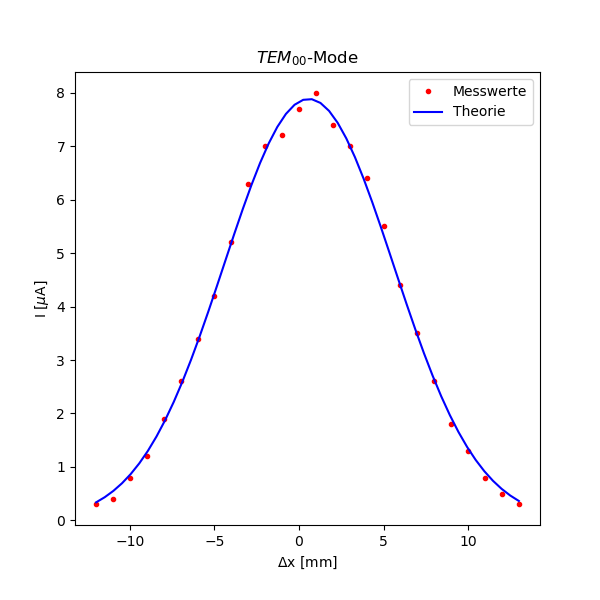
\includegraphics{figures/TEM_00.png}
\caption{Messung und theoretische Werte der $\text{TEM}_{00}$}
\label{fig:TEM_00}
\end{figure}


\begin{figure}
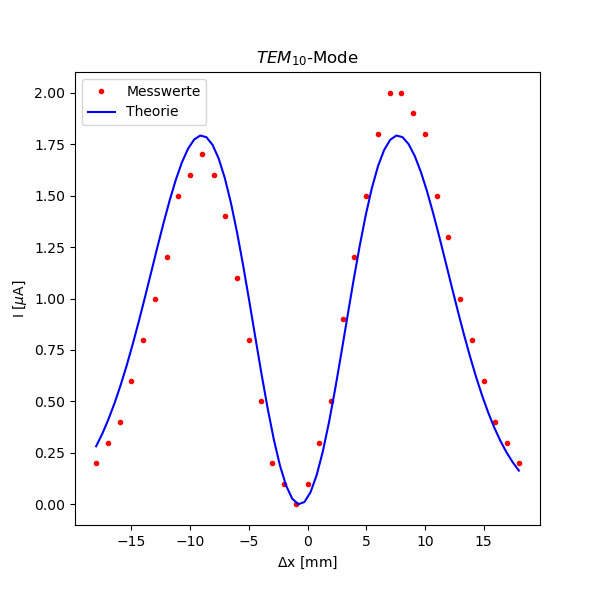
\includegraphics{figures/TEM_10.png}
\caption{Messung und theoretische Werte der $\text{TEM}_{10}$}
\label{fig:TEM_10}
\end{figure}




\begin{figure}
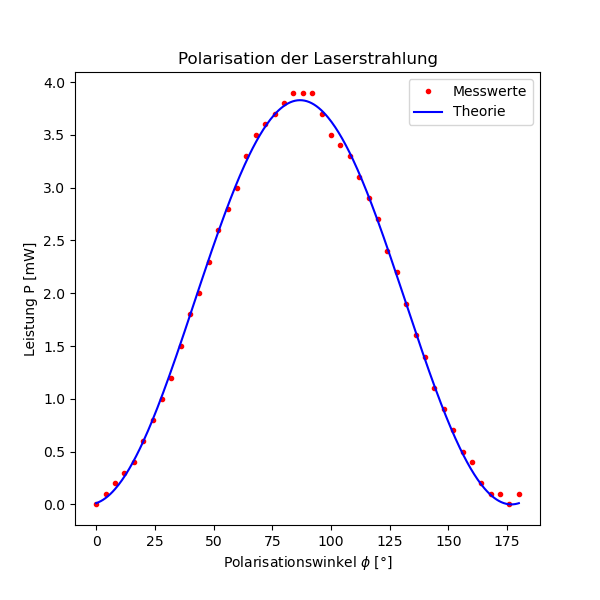
\includegraphics{figures/Polarisation.png}
\caption{Messung und theoretische Werte der Polarisation des Laserstrahls}
\label{fig:Polarisation}
\end{figure}





\begin{figure}
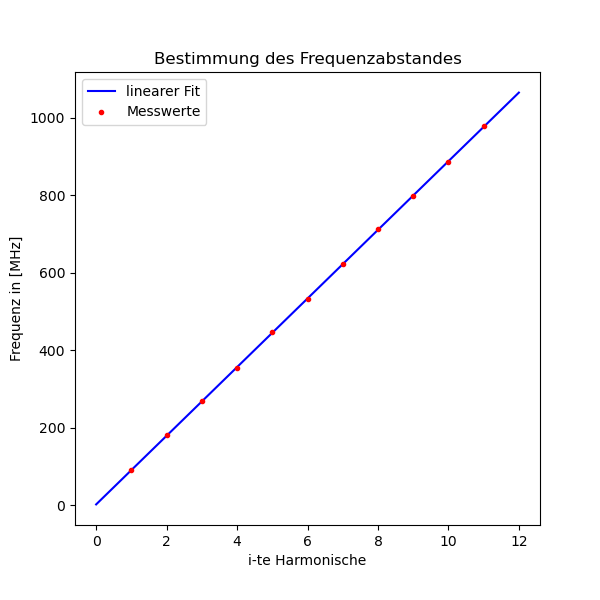
\includegraphics{figures/Frequenzabstand.png}
\caption{Gemessene Schwebungsfrequenzen und linearer Fit zur Resonatorlänge $L = 167,6\,\text{cm}$}
\label{fig:linMultimoden}
\end{figure}



\begin{figure}
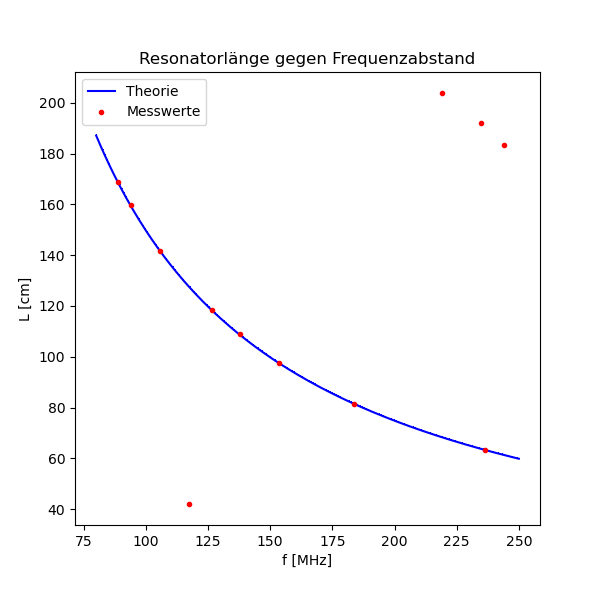
\includegraphics{figures/Multimoden.png}
\caption{Resonatorlänge $L$ und Abstand zweier longitudinaler Moden $f$: Messwerte und theoretische Werte}
\label{fig:Multimoden}
\end{figure}




\section{Tabellen}


\begin{table}
\centering
\caption{Maximale stabile Resonatorlängen L für Spiegel mit Krümmungsradius $r_1$ und $r_2$}
\begin{tabular}{c c c}
\toprule
{$L$[cm]} & {$r_1$[mm]} & {$r_2$[mm]}\\
\midrule
204,0  &  1400 & 1400\\
139,5  &  $\infty$ & 1400\\
\bottomrule
\label{tab:maximale Resonatorlängen}
\end{tabular}
\end{table}




\begin{table}
\centering
\caption{Messung der Intensitätsverteilung in Einheiten der Stromstärke zur $\text{TEM}_{00}$}
\begin{tabular}{c c}
\toprule
{$\Delta x$[mm]} & {$I$[$\mu$A]}\\
\midrule
-12	&	0,3	\\
-11	&	0,4	\\
-10	&	0,8	\\
-9	&	1,2	\\
-8	&	1,9	\\
-7	&	2,6	\\
-6	&	3,4	\\
-5	&	4,2	\\
-4	&	5,2	\\
-3	&	6,3	\\
-2	&	7,0	\\
-1	&	7,2	\\
0	&	7,2	\\
1	&	8,0	\\
2	&	7,4	\\
3	&	7,0	\\
4	&	6,4	\\
5	&	5,5	\\
6	&	4,4	\\
7	&	3,5	\\
8	&	2,6	\\
9	&	1,8	\\
10	&	1,3	\\
11	&	0,8	\\
12	&	0,5	\\
13	&	0,3	\\
\bottomrule
\label{tab:TEM_00}
\end{tabular}
\end{table}

\begin{table}
\centering
\caption{Messung der Intensitätsverteilung in Einheiten der Stromstärke zur $\text{TEM}_{10}$}
\begin{tabular}{c c}
\toprule
{$\Delta x$[mm]} & {$I$[$\mu$A]}\\
\midrule
-18	&	0,2	\\
-17	&	0,3	\\
-16	&	0,4	\\
-15	&	0,6	\\
-14	&	0,8	\\
-13	&	1,0	\\
-12	&	1,2	\\
-11	&	1,5	\\
-10	&	1,6	\\
-9	&	1,7	\\
-8	&	1,6	\\
-7	&	1,2	\\
-6	&	1,1	\\
-5	&	0,8	\\
-4	&	0,5	\\
-3	&	0,2	\\
-2	&	0,1	\\
-1	&	0,0	\\
0	&	0,1	\\
1	&	0,3	\\
2	&	0,5	\\
3	&	0,9	\\
4	&	1,2	\\
5	&	1,5	\\
6	&	1,8	\\
7	&	2,0	\\
8	&	2,0	\\
9	&	1,9	\\
10	&	1,8	\\
11	&	1,5	\\
12	&	1,3	\\
13	&	1,0	\\
14	&	0,8	\\
15	&	0,6	\\
16	&	0,5	\\
17	&	0,4	\\
18	&	0,2	\\
\bottomrule
\label{tab:TEM_10}
\end{tabular}
\end{table}





\begin{table}
\centering
\caption{gemessene Strahlungsleistung $P$ zu verschiedenen Polarisationswinkeln $\phi$}
\begin{tabular}{c c c c}
\toprule
{$\phi$[°]} & {$P$[mW]} & {$\phi$[°]} & {$P$[mW]}\\
\midrule
0	&	0,0	&	92	&	3,9	\\
4	&	0,1	&	96	&	3,7	\\
8	&	0,2	&	100	&	3,5	\\
12	&	0,3	&	104	&	3,4	\\
16	&	0,4	&	108	&	3,3	\\
20	&	0,6	&	112	&	3,1	\\
24	&	0,8	&	116	&	2,9	\\
28	&	1,0	&	120	&	2,7	\\
32	&	1,2	&	124	&	2,4	\\
36	&	1,5	&	128	&	2,2	\\
40	&	1,8	&	132	&	1,9	\\
44	&	2,0	&	136	&	1,6	\\
48	&	2,3	&	140	&	1,4	\\
52	&	2,6	&	144	&	1,1	\\
56	&	2,8	&	148	&	0,9	\\
60	&	3,0	&	152	&	0,8	\\
64	&	3,3	&	156	&	0,5	\\
68	&	3,5	&	160	&	0,4	\\
72	&	3,6	&	164	&	0,2	\\
76	&	3,7	&	168	&	0,1	\\
80	&	3,8	&	172	&	0,1	\\
84	&	3,9	&	176	&	0,0	\\
88	&	3,9	&	180	&	0,1	\\
\bottomrule
\label{tab:Polarisation}
\end{tabular}
\end{table}




\begin{table}
\centering
\caption{Schwebungsfrequenzen $\nu_i$ zu verschiedenen Resonatorlängen $L$}
\begin{tabular}{c c c c c c c}
\toprule
$L$ [cm]	&	202,6	&	190,7	&	182,0	&	167,6	&	158,2	&	140,4	\\
\midrule
$\nu_1$[MHz]	&	225	&	233	&	244	&	90	&	94	&	105	\\
$\nu_2$[MHz]	&	443	&	469	&	495	&	180	&	188	&	214	\\
$\nu_3$[MHz]	&	664	&	701	&	730	&	270	&	285	&	319	\\
$\nu_4$[MHz]	&	881	&	938	&	979	&	353	&	375	&	424	\\
$\nu_5$[MHz]	&		&		&		&	446	&	473	&	529	\\
$\nu_6$[MHz]	&		&		&		&	533	&	566	&	634	\\
$\nu_7$[MHz]	&		&		&		&	623	&	660	&	739	\\
$\nu_8$[MHz]	&		&		&		&	713	&	750	&	844	\\
$\nu_9$[MHz]	&		&		&		&	799	&	844	&	953	\\
$\nu_{10}$[MHz]	&		&		&		&	885	&	941	&	1058	\\
$\nu_{11}$[MHz]	&		&		&		&	979	&	1035	&	1163	\\
&		&		&		&		&		&\\
											\midrule		
&		&		&		&		&		&\\		
$L$ [cm]	&	116,9	&	107,4	&	96,2	&	80,2	&	61,8	&	40,5	\\
\midrule
$\nu_1$[MHz]	&	128	&	139	&	154	&	184	&	236	&	90	\\
$\nu_2$[MHz]	&	255	&	278	&	311	&	368	&	473	&	270	\\
$\nu_3$[MHz]	&	383	&	416	&	461	&	551	&	709	&	360	\\
$\nu_4$[MHz]	&	506	&	551	&	615	&	735	&	945	&	446	\\
$\nu_5$[MHz]	&	634	&	690	&	769	&	919	&		&	630	\\
$\nu_6$[MHz]	&	761	&	829	&	923	&	1103	&		&	716	\\
$\nu_7$[MHz]	&	889	&	968	&	1076	&		&		&	799	\\
$\nu_8$[MHz]	&	1013	&	1103	&	1230	&		&		&		\\
$\nu_9$[MHz]	&		&		&		&		&		&		\\
$\nu_{10}$[MHz]	&		&		&		&		&		&		\\
$\nu_{11}$[MHz]	&		&		&		&		&		&		\\

\bottomrule
\label{tab:Multimoden}
\end{tabular}
\end{table}





\begin{table}
\centering
\caption{Parameter der linearen Regression}
\begin{tabular}{c c}
\toprule

{$m$[MHz]}&{$n$[MHz]}\\
\midrule
{ 218,899 \pm 0,232 }& { 6,000 \pm 0,636 }\\
{ 234,699 \pm 0,293 }& { -1,499 \pm 0,803 }\\
{ 243,999 \pm 0,959 }& { 2,000 \pm 2,627 }\\
{ 88,627 \pm 0,188 }& { 1,963 \pm 1,275}\\
{ 93,918 \pm 0,170 }& { 1,127 \pm 1,153}\\
{ 105,618 \pm 0,121 }& { 1,018 \pm 0,822 }\\
{ 126,511 \pm 0,153 }& { 1,821 \pm 0,774 }\\
{ 137,809 \pm 0,154 }& { 1,607 \pm 0,778 }\\
{ 153,535 \pm 0,145 }& { 1,464 \pm 0,732 }\\
{ 183,771 \pm 0,049 }& { 0,133 \pm 0,191 }\\
{ 236,300 \pm 0,035 }& { 0,000 \pm 0,098 }\\
{ 117,464 \pm 4,238 }& { 3,143 \pm 18,955 }\\

\bottomrule
\label{tab:linMultimoden}
\end{tabular}
\end{table}





\begin{table}
\centering
\caption{Abstände der Beugungsmaxima für zwei verschiedene Gitter}
\begin{tabular}{c c}
\toprule
$100\,$lines/mm&$600\,$lines/mm\\
$\delta x$[cm]&$\delta x$[cm]\\
\midrule
2,1	&	22,9	\\
2,1	&	22,9	\\
2,1	&		\\
2,1	&		\\
2,1	&		\\
2,1	&		\\
\bottomrule
\label{tab:WellenAbstand}
\end{tabular}
\end{table}






























































